% Drawing 148/01-15 -- folder 148, batch 01, archive page 18 (PDF page 19).
% Transcription: en haut à droite, une sphère : l'équateur à l'encre (l'arrière en pointillé) portant quatre points, deux à l'avant et deux à l'arrière ; deux grands cercles méridiens passant chacun par un point de l'avant et un point de l'arrière, en vert et en brun, les moitiés arrière en pointillé ou en tirets ; de petites flèches le long des méridiens.
% Kind: sphere with equator, four points and two meridian circles with arrows. Method 2 (schematic redraw from the facsimile). Status: partial.
% Notes: Colour render of p. 18. Faint pencil outline (drawn pencil). Equator in black ink, front half solid, back half dotted, with two dots on the front and two on the back, each placed on the ellipse. Two meridian circles through the poles: the first through the front-left and the back-right points (front half brown above the equator and heavy green below; back half brown dashes above, green dots below), the second through the front-right and the back-left points (front half heavy green above and brown below; back half green dots above, brown dashes below). Eight small arrow-like marks sit along the meridians, one on each half above and below the equator; they are drawn as short downward arrows. Still differs: the direction of the small arrows is a reading (they are blots on the page), and the alternation of green and brown follows the crop approximately. Redrawn 2026-11-12 (issue 128): to check again.
% Coordinates: 1 unit = 1 mm = 1/100 of the crop width, y downwards as on the crop (bbox in page fractions: [0.44, 0.115, 0.72, 0.31]).
% Redrawn by Claude (claude-fable-5-2), issue #128, 2026-11-12; not checked by a human; not compiled (no TeX in the session).
% Rights: reproduces part of the work -- behind RENDER_TRANSCRIPTS, never published by itself.
\documentclass[tikz,border=3pt]{standalone}
\usepackage{amsmath,amssymb}
\usetikzlibrary{patterns,arrows.meta}
\tikzset{pencil/.style={black!45}, struck/.style={black!35}, mpt/.style={circle,draw,inner sep=1.3pt}, pt/.style={circle,fill,inner sep=0.9pt}, opt/.style={circle,draw,fill=white,inner sep=1.1pt}, Rd/.style={red!75!black}, Gn/.style={green!45!black}, Br/.style={brown!70!black}}
\begin{document}
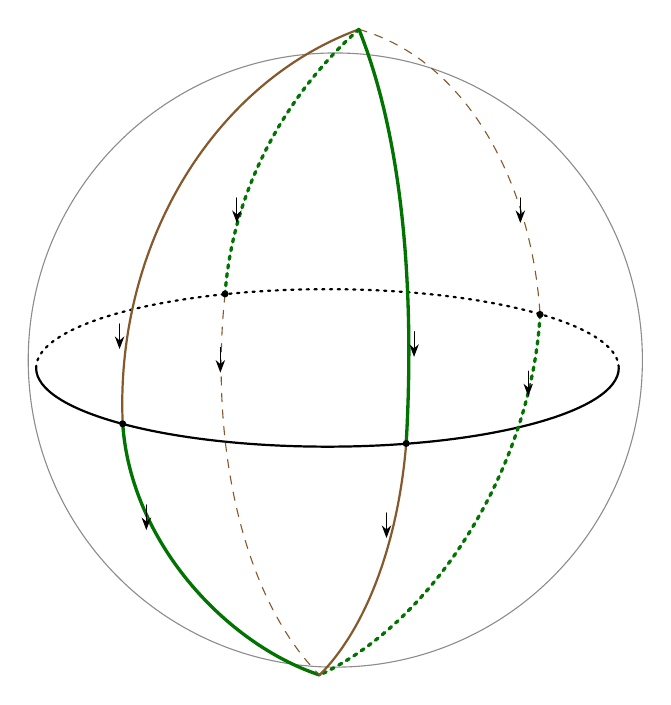
\begin{tikzpicture}[x=1mm,y=-1mm,line cap=round,line join=round,font=\small]
\draw[pencil] (52,52) circle [radius=39];
\coordinate (N) at (55,10);
\coordinate (S) at (50,92);
\coordinate (fl) at (25,60.1);
\coordinate (fr) at (61,62.6);
\coordinate (bl) at (38,43.6);
\coordinate (br) at (78,46.2);
\draw[thick] (14,53) arc [start angle=180, end angle=0, x radius=37, y radius=10];
\draw[dotted,thick] (14,53) arc [start angle=180, end angle=360, x radius=37, y radius=10];
\draw[Br,thick] (N) .. controls (36,17) and (24,38) .. (fl);
\draw[Gn,very thick] (fl) .. controls (26,75) and (38,88) .. (S);
\draw[Br,dashed] (N) .. controls (69,14) and (77,30) .. (br);
\draw[Gn,dotted,very thick] (br) .. controls (77,65) and (65,85) .. (S);
\draw[Gn,very thick] (N) .. controls (61,25) and (62,45) .. (fr);
\draw[Br,thick] (fr) .. controls (60,75) and (56,86) .. (S);
\draw[Gn,dotted,very thick] (N) .. controls (46,18) and (39,30) .. (bl);
\draw[Br,dashed] (bl) .. controls (36,62) and (40,82) .. (S);
\node[pt] at (fl) {};
\node[pt] at (fr) {};
\node[pt] at (bl) {};
\node[pt] at (br) {};
\foreach \x/\y in {24.6/49, 39.5/33, 37.4/52, 62/50, 75.5/33, 76.5/55, 28/72, 58.5/73} {
\draw[-{Stealth[length=1.6mm]}] (\x,\y-1.6) -- (\x,\y+1.6);
}
\end{tikzpicture}
\end{document}
